%!TeX root = free_rtos
\documentclass[../main.tex]{subfiles}

\begin{document}
    \section{FreeRTOS}
    
    FreeRTOS is an open-source real-time operating system for microcontroller. It is available for many platforms such as arduino, mbed, espressif, etc., and widely used in industrial, medical, automotive sectors. Even though the MCU is single-core, the firmware will run tasks with asynchronous and synchronous component, and FreeRTOS will be essential.
    
    \pagebreak
    \section{Firmware's flowchart}

    The following diagram is the main program's flowchart:

    \begin{figure}[!h]
        \centerline{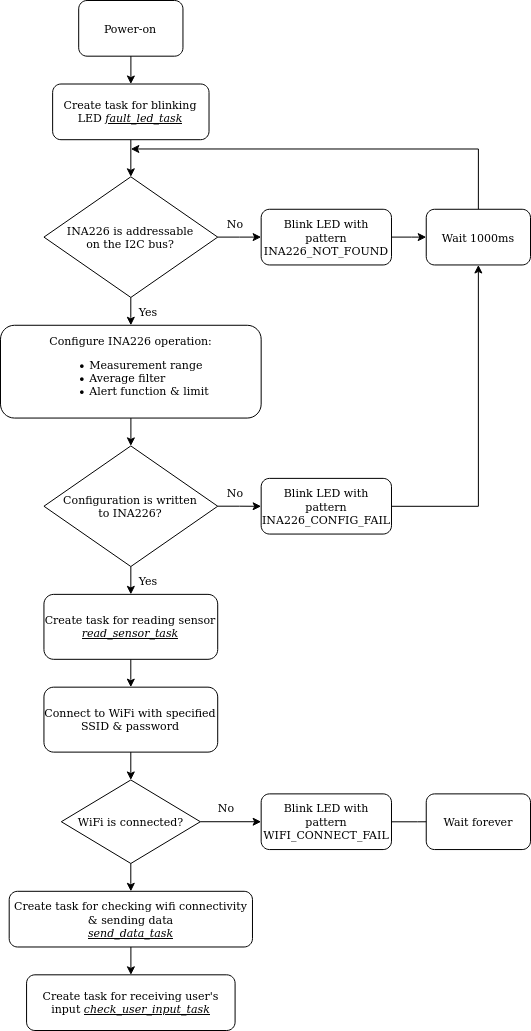
\includegraphics[scale=0.56]{media/main_program_flowchart.drawio.png}}
        \caption{Main program's flowchart.}
        \label{fig:main_program_flowchart}
    \end{figure}

    \justify
    The following code snippet is the setup function in the MCU, executing the above flowchart.
    \lstinputlisting[language=C++]{setup.cpp}

    \pagebreak
    \subsection{\textit{read\_sensor\_task}}
    The following diagram is the \textit{read\_sensor\_task}'s flowchart.

    \begin{figure}[!h]
        \centerline{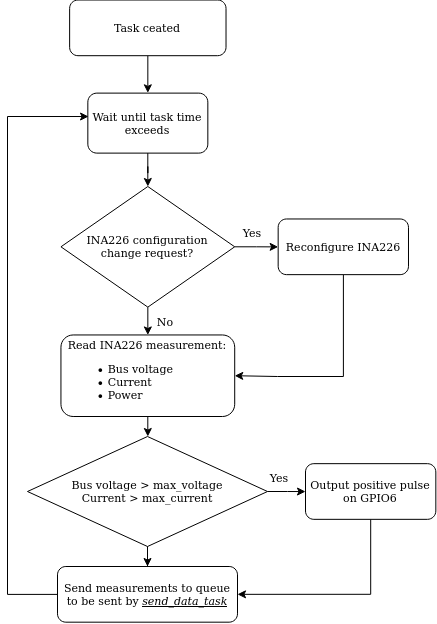
\includegraphics[scale=0.6]{media/read_sensor_task_flowchart.drawio.png}}
        \caption{Read sensor task flowchart.}
        \label{fig:read_sensor_task_flowchart}
    \end{figure}

    \begin{enumerate}
        \item The task will continuously read the measurements from the INA226 sensor board, compare the values with the user-defined maximum values, and outputs a positive pulse to turn off the MOSFET when a maximum value is exceeded.
        \item The task will wait for a semaphore to be set when the user requests an INA226 configuration change, then update the maximum values and reconfigure the INA226 accordingly.
    \end{enumerate}

    \pagebreak
    \justify
    The following code snippet is the \textit{read\_sensor\_task} function in the MCU, executing the above flowchart.
    \lstinputlisting[language=C++]{read_sensor_task.cpp}

    \pagebreak
    \subsection{\textit{send\_data\_task}}
    The following diagram is the \textit{send\_data\_task}'s flowchart.

    \begin{figure}[!h]
        \centerline{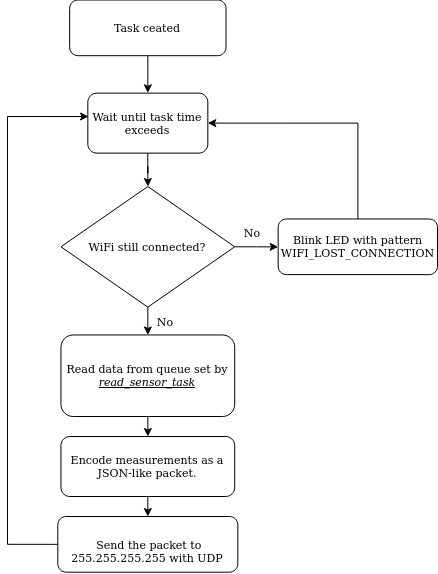
\includegraphics[scale=0.55]{media/send_data_task_flowchart.drawio.png}}
        \caption{Send data task flowchart.}
        \label{fig:send_data_task_flowchart}
    \end{figure}
    
    \begin{enumerate}
        \item WiFi connectivity is checked before sending the data to the application. If the WiFi connection is lost, blink LED signaling the error.
        \item The measured data is encoded into a JSON-like string. The format is: \newline \centerline{${data}_0={value}_0\&{data}_1={value}_1\&...\&{data}_n={value}_n$.}\newline Then, the encoded string is sent to 255.255.255.255 with UDP protocol. This will broadcast to every device in the local network including, of course, the user's device.
    \end{enumerate}

    \pagebreak
    \justify
    The following code snippet is the \textit{send\_data\_task} function in the MCU, executing the above flowchart.
    \lstinputlisting[language=C++]{send_data_task.cpp}

    \pagebreak
    \subsection{\textit{check\_user\_input\_task}}
    The following diagram is the \textit{check\_user\_input\_task}'s flowchart.

    \begin{figure}[!h]
        \centerline{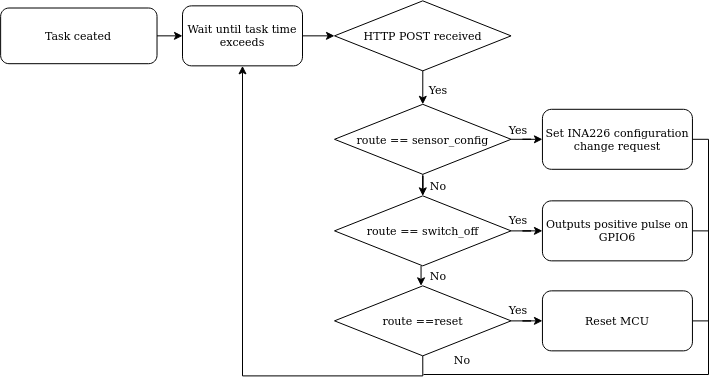
\includegraphics[scale=0.55]{media/check_user_input_task_flowchart.drawio.png}}
        \caption{Send data task flowchart.}
        \label{fig:check_user_input_task_flowchart}
    \end{figure}
    
    \justify
    The task wait for a HTTP POST request from the user, checks the route and execute the following:

    \begin{itemize}
        \item sensor\_config: Set the semaphore that alerts the \textit{read\_data\_task} to update the INA226 configuration.
        \item switch\_off: Outputs a positive pulse on GPIO6 turning the MOSFET switch off.
        \item reset: Reset the MCU.
    \end{itemize}

    \pagebreak
    \justify
    The following code snippet is the \textit{check\_user\_input\_task} function in the MCU, executing the above flowchart.
    \lstinputlisting[language=C++]{check_user_input_task.cpp}


    

\end{document}